% !TeX spellcheck = pt_PT2

\chapter{Implementação}
\label{ch:implementacao}

Neste capítulo, a implementação é analisada em duas vertentes complementares.  
Na primeira parte, dedicada ao \emph{hardware}, descreve-se a plataforma de desenvolvimento na Secção~\ref{sec:plataforma-desenvolvimento}, seguida da integração dos propulsores na Subsecção~\ref{subsec:integracao-propulsores}, da utilização dos sensores na Subsecção~\ref{subsec:sensores}, dos módulos de comunicação e, por fim, da conceção da \gls{pcb} na Subsecção~\ref{subsec:pcb}. Na segunda parte, referente ao \emph{software}, detalham-se a arquitetura modular do código na Subsecção~\ref{subsec:arquitetura-codigo}, os mecanismos de controlo de motores na Subsecção~\ref{subsec:controlo-de-motores}, a aquisição e processamento de dados dos sensores na Subsecção~\ref{subsec:processamento-sensores} e as estratégias de comunicação via \gls{lora} na Subsecção~\ref{subsec:comunicacao-lora}. Esta organização permite compreender de forma clara e sistemática como os diferentes componentes foram concebidos e integrados para dar origem ao sistema ciberfísico proposto.

\section{Plataforma de Desenvolvimento}
\label{sec:plataforma-desenvolvimento}

A plataforma de desenvolvimento utilizada neste trabalho constitui a base para a implementação tanto de \emph{hardware} como de \emph{software}, garantindo a integração eficiente de todos os módulos do sistema. Nesta secção são apresentados dois elementos fundamentais: em primeiro lugar, o microcontrolador \gls{esp32}, descrito na Subsecção~\ref{subsec:esp32}, que assegura o processamento central e a coordenação das interfaces de comunicação; e, em segundo lugar, o ambiente de programação, detalhado na Subsecção~\ref{subsec:ambiente-programacao}, que fornece as ferramentas necessárias para a compilação, gestão de bibliotecas e controlo de versões do código. A análise conjunta destes componentes evidencia como a escolha da plataforma contribuiu para a robustez, modularidade e escalabilidade do protótipo desenvolvido.


\subsection{Microcontrolador \acrfull{esp32}}
\label{subsec:esp32}

O microcontrolador \acrfull{esp32} é um sistema de elevado desempenho e reduzidas dimensões, dotado de um processador \emph{dual-core} com frequência até 240 MHz e suporte a vírgula flutuante. Esta capacidade de processamento é largamente superior às necessidades do presente projeto, garantindo margem para futuras expansões e algoritmos mais exigentes em termos de cálculo.  

Para a implementação descrita nesta \gls{tfm} foi utilizado o módulo TTGO \gls{lora}32, representado na Figura \ref{fig:lora32}, que integra num único dispositivo o microcontrolador \gls{esp32}, um transceptor (transmite e recebe sinais) \gls{lora} e um \emph{display} \gls{oled} de 0.96 polegadas. Esta integração reduz significativamente a complexidade do \emph{\emph{hardware}}, uma vez que combina num só módulo os principais elementos de computação e comunicação necessários para o funcionamento do \gls{usv}.  

\begin{figure}[H]
    \centering
    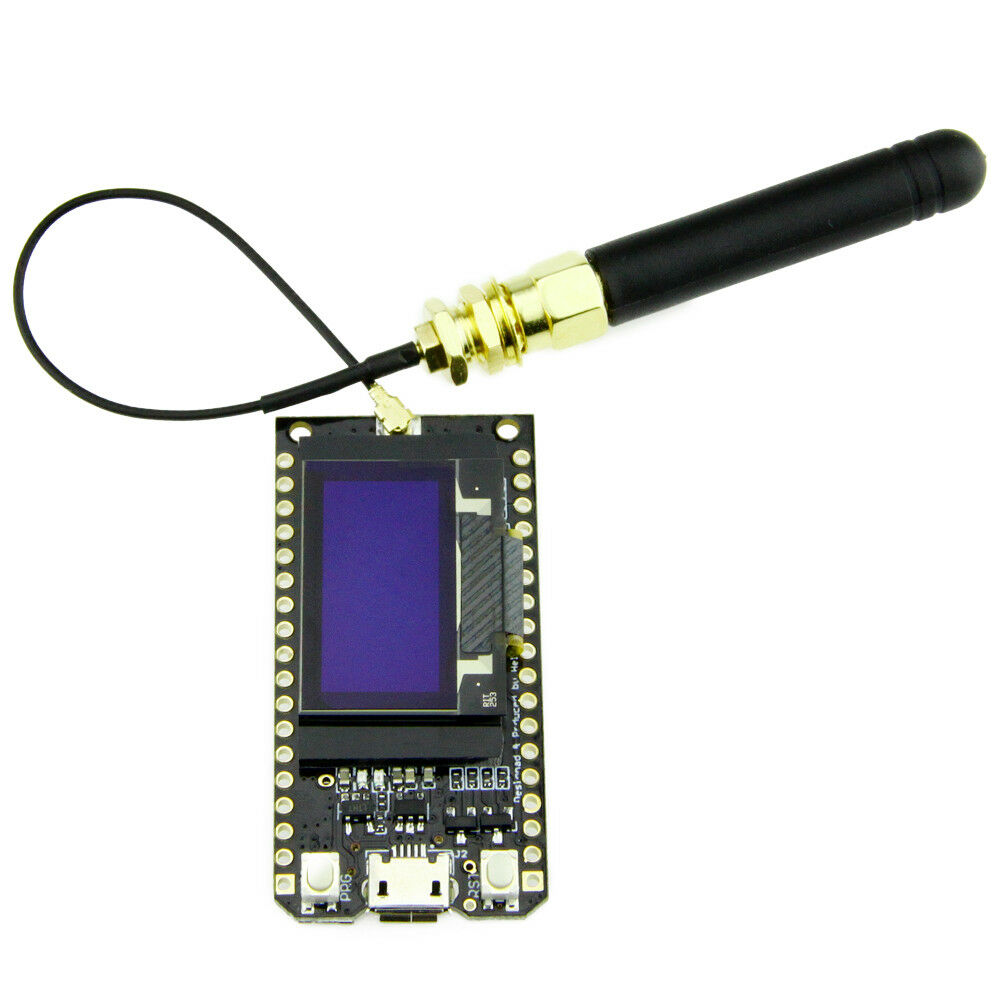
\includegraphics[width=0.33\linewidth]{figuras/lora32.png}
    \caption{\gls{esp32} TTGO \gls{lora}32}
    \label{fig:lora32}
\end{figure}

Do ponto de vista das interfaces de comunicação, o \gls{esp32} suporta nativamente \gls{i2c}, \gls{uart} e \gls{spi}, além da geração de sinais \gls{pwm}, o que o torna adequado para aplicações de controlo de atuadores e aquisição de dados de sensores heterogéneos. O módulo disponibiliza também conectividade sem fios através de \gls{wifi} e \emph{bluetooth}, que, embora não tenham sido utilizados diretamente neste trabalho, representam uma mais-valia para cenários futuros, como a monitorização remota via redes locais ou a configuração simplificada de parâmetros através de dispositivos móveis.  

O \emph{display} \gls{oled} incorporado revelou-se particularmente útil durante a fase de testes e validação, ao permitir monitorizar em tempo real o estado do sistema. Através dele foi possível confirmar a receção de dados provenientes de sensores, a correta execução de comandos de controlo e a integridade das mensagens trocadas via \gls{lora}. Este recurso facilitou o processo de \emph{debug} e reduziu a dependência de sistemas de monitorização externos, acelerando a fase de desenvolvimento.  

Outro aspeto relevante é a vasta comunidade de suporte e o ecossistema de bibliotecas disponíveis para o \gls{esp32}, tanto no ambiente Arduino como em \emph{frameworks} mais avançadas, como a \gls{esp-idf}, que constitui a framework oficial de desenvolvimento disponibilizada pela Espressif programável em C. Esta característica contribui para uma maior fiabilidade no desenvolvimento, reduzindo riscos de integração e permitindo concentrar o esforço na implementação da arquitetura modular proposta para o \gls{usv}.

Em síntese, o módulo TTGO \gls{lora}32 constituiu uma plataforma robusta, versátil e de fácil integração, adequando-se não apenas às exigências do desenvolvimento deste protótipo de \gls{usv}, mas também oferecendo capacidade de evolução para cenários mais complexos, como a execução de algoritmos de navegação autónoma em tempo real ou a integração com sistemas de monitorização distribuídos.

\subsection{Ambiente de Programação}
\label{subsec:ambiente-programacao}

O desenvolvimento do \emph{software} para o protótipo do \gls{usv} foi realizado recorrendo ao ambiente de programação PlatformIO, integrado no editor Visual Studio Code. Esta escolha deve-se às vantagens oferecidas pelo PlatformIO, nomeadamente a gestão centralizada de bibliotecas e o controlo de versões das mesmas, a configuração automatizada do ambiente de compilação e a possibilidade de integração com múltiplos \emph{frameworks} de desenvolvimento.  

Um exemplo claro destas funcionalidades pode ser observado no ficheiro de configuração \texttt{platformio.ini}. Este ficheiro define todas as dependências e parâmetros necessários para compilar e carregar o projeto, assegurando que qualquer programador envolvido no desenvolvimento utiliza exatamente as mesmas versões de bibliotecas e definições de compilação. A Listagem \ref{lst:platformio} mostra um exemplo de um ficheiro de configuração do PlatformIO.

\lstinputlisting[caption={Exemplo de ficheiro \texttt{platformio.ini} utilizado no projeto}, label={lst:platformio}, style=BetterCPP]{code/minimal/exampleplatformIO.ini}

Neste caso, a secção \texttt{[env:ttgo-lora32-v1]} especifica o ambiente de compilação direcionado para a placa TTGO \gls{lora}32, fixando a versão da plataforma \gls{esp32} (\texttt{espressif32@$\sim$5.0.0}) e o \emph{framework} (\texttt{arduino}). A diretiva \texttt{lib\_deps} lista todas as bibliotecas necessárias ao projeto, juntamente com a versão exata de cada uma. Assim, bibliotecas como \texttt{Adafruit SSD1306}, \texttt{LoRa} ou \texttt{TinyGPSPlus} são automaticamente descarregadas e mantidas consistentes em qualquer máquina de desenvolvimento, evitando problemas de incompatibilidade entre versões.  

Este mecanismo garante que o projeto é reprodutível e portável, pois basta clonar o repositório e executar a compilação para obter um ambiente idêntico, sem necessidade de configurar manualmente as bibliotecas ou dependências.

No âmbito deste projeto, foi utilizada a \emph{framework} Arduino do PlatformIO, pela sua simplicidade e pela ampla disponibilidade de bibliotecas compatíveis com o \gls{esp32}. Alternativamente, o \gls{esp-idf} poderia ter sido utilizado, oferecendo maior controlo de baixo nível e otimizações de desempenho, mas a sua maior complexidade tornaria o ciclo de desenvolvimento menos ágil. Assim, a opção pelo ecossistema Arduino mostrou-se mais adequada à prototipagem rápida e à integração de múltiplos sensores e interfaces de comunicação.  

Para além destas ferramentas, foi também utilizado o sistema de controlo de versões Git, com integração em repositório remoto público (\emph{open source}) no GitHub \cite{github-usv}. Este processo assegurou a rastreabilidade das alterações, a organização das diferentes versões do código e a possibilidade de colaboração futura.  

Embora o desenvolvimento principal tenha sido efetuado no Visual Studio Code com o suporte do PlatformIO, foram também realizados testes complementares na Arduino IDE, devido à sua simplicidade na programação inicial do \gls{esp32} e na verificação rápida da compatibilidade das bibliotecas utilizadas.  

Em síntese, a combinação destas ferramentas permitiu estabelecer um ambiente de desenvolvimento robusto, flexível e adaptado às exigências do projeto, ao mesmo tempo que garantiu escalabilidade e reprodutibilidade para trabalhos futuros.

\section{Implementação de \emph{Hardware}}
\label{sec:implementacao-hardware}

A implementação do \emph{\emph{hardware}} do sistema desenvolvido nesta \gls{tfm} assenta numa arquitetura modular, representada de forma esquemática na Figura \ref{fig:placeholder}. Tal como no projeto realizado em \cite{didactic-robot-thesis}, procurou-se manter uma estrutura clara e escalável, onde cada componente desempenha um papel bem definido e comunica com a unidade central de forma eficiente.  

O núcleo do sistema é constituído pelo microcontrolador \gls{esp32}, responsável por coordenar a execução das tarefas de controlo, comunicação e aquisição de dados. Através do barramento \gls{i2c}, o \gls{esp32} comunica com um expansor, responsável pela distribuição dos sinais de controlo e pela interface com os diferentes periféricos \gls{pwm}. Este dispositivo disponibiliza 16 canais adicionais de saída a partir de apenas dois pinos de comunicação \gls{i2c} (SDA e SCL), sendo ainda possível encadear múltiplos expansores para aumentar o número de canais disponíveis. Esta solução permite ultrapassar a limitação do número de pinos físicos do microcontrolador, assegurando a escalabilidade do sistema e reduzindo simultaneamente a complexidade das interligações elétricas, o que simplifica a integração de novos módulos funcionais.

Esta representação global serve como ponto de partida para a descrição detalhada apresentada nas subseções seguintes, onde são abordadas individualmente a integração dos propulsores, a utilização dos sensores, os módulos de comunicação e a conceção da \gls{pcb}.

\subsection{Integração dos Propulsores}
\label{subsec:integracao-propulsores}

A propulsão do \gls{usv} é assegurada por dois propulsores elétricos independentes, cada um alimentado por uma bateria dedicada de 12 V. Esta configuração garante uma fonte de energia estável e suficientemente dimensionada para fornecer a corrente necessária ao funcionamento contínuo dos motores, reduzindo simultaneamente o risco de sobrecarga caso ambos fossem alimentados por uma única bateria.  

A descrição detalhada das características dos motores e do respetivo sistema de controlo eletrónico encontra-se apresentada na Secção \ref{sec:motor}, enquanto o princípio de funcionamento dos \gls{esc} é explicado na Secção \ref{sec:esc}. Aqui, foca-se a forma como esses componentes foram efetivamente integrados no protótipo desenvolvido.  

Cada propulsor encontra-se ligado ao respetivo \gls{esc}, responsável por converter os sinais de controlo recebidos em impulsos elétricos adequados ao motor \emph{brushless}. Tal como descrito anteriormente, o controlo é realizado por sinais de \gls{pwm}, sendo que, no protótipo implementado, o propulsor esquerdo foi ligado ao canal 14 do expansor, enquanto o propulsor direito foi associado ao canal 15. Apesar desta atribuição, qualquer outro canal disponível poderia ser utilizado, uma vez que a correspondência é definida ao nível do \emph{software}.  

O funcionamento dos motores segue o princípio explicado na Secção \ref{sec:esc}, em que a largura do pulso de \gls{pwm} define o sentido e a intensidade da rotação. Esta abordagem permite um controlo independente de cada propulsor, possibilitando tanto movimentos de translação em linha reta como manobras de rotação em torno do próprio eixo, aumentando significativamente a manobrabilidade da embarcação.  

No que respeita aos testes, cada motor foi inicialmente verificado de forma individual, em conjunto com o seu respetivo \gls{esc}, assegurando a correta resposta a diferentes larguras de pulso, a ausência de falhas de comunicação e a estabilidade térmica durante o funcionamento contínuo. Apenas após a validação isolada de cada propulsor se procedeu à sua integração conjunta no sistema, confirmando a coerência do funcionamento em paralelo e a capacidade de executar manobras de coordenação.  

Esta estratégia de integração modular e progressiva assegura que cada propulsor pode ser controlado e validado de forma independente, ao mesmo tempo que garante a escalabilidade do sistema, permitindo a futura adição de mais motores ou a substituição dos atuais sem alterações significativas à arquitetura global.

\subsection{Sensores}
\label{subsec:sensores}

Nesta subseção são descritos os principais sensores integrados no \gls{usv}, responsáveis pela recolha de dados de navegação e monitorização ambiental. São apresentados o \gls{imu}, para determinação do \emph{yaw}, \emph{pitch} e \emph{roll}, e o módulo \gls{gps}, para aquisição de posição geográfica. Adicionalmente, discutem-se aspetos de integração elétrica e física relevantes para o funcionamento estável do sistema.

\subsubsection{\acrfull{imu}}

Para a determinação do \emph{yaw}, \emph{pitch} e \emph{roll} do \gls{usv}, foi utilizado um \gls{imu} baseado no sensor ICM-20948, ilustrado na Figura \ref{fig:imu}. Este dispositivo integra num único chip um acelerómetro de três eixos, um giroscópio de três eixos e um magnetómetro de três eixos, totalizando nove graus de liberdade (9-DOF \emph{gyro-stabilized eCompass} \cite{9dof}). 

\begin{figure}[H]
    \centering
    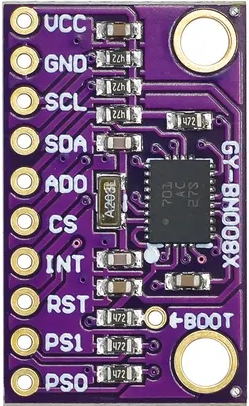
\includegraphics[width=0.25\linewidth]{figuras/imu-icm.jpg}
    \caption{\gls{imu} ICM-20948 utilizada no protótipo}
    \label{fig:imu}
\end{figure}

A combinação destes sensores permite medir acelerações lineares, taxas de rotação e intensidade do campo magnético terrestre, fornecendo assim dados fundamentais para o cálculo do \emph{yaw},  \emph{pitch} e \emph{roll}.

Em termos de integração física, o módulo \gls{imu} foi ligado ao microcontrolador \gls{esp32} através do barramento \gls{i2c}, utilizando os pinos SDA e SCL. No protótipo, foram atribuídos os pinos GPIO 21 (SDA) e GPIO 22 (SCL), respetivamente, recorrendo a uma frequência de comunicação de 400 kHz (\emph{I2C Fast Mode}). Esta interface garante uma comunicação fiável e de elevada velocidade, adequada para a leitura periódica dos dados dos nove eixos.

O ICM-20948 suporta dois endereços \gls{i2c} distintos (0x68 e 0x69), selecionáveis via configuração de \emph{hardware}, o que possibilita a integração simultânea de múltiplos módulos no mesmo barramento, caso seja necessário. No presente projeto, foi utilizada a configuração por omissão (0x68).  

A ligação elétrica do módulo foi realizada diretamente à linha regulada de 3.3~V fornecida pelo \gls{esp32}, estabelecendo-se também a referência comum de massa (GND). Esta configuração garante compatibilidade elétrica entre os dispositivos e elimina a necessidade de conversores de nível lógico, uma vez que tanto o \gls{esp32} como o ICM-20948 operam nativamente a 3.3~V.

O módulo foi montado em proximidade com a unidade de processamento central, dentro da caixa estanque, de forma a reduzir o comprimento dos cabos e minimizar a suscetibilidade a ruídos elétricos. A posição física do sensor foi escolhida de modo a manter o alinhamento dos seus eixos com a estrutura da embarcação, simplificando assim a interpretação dos dados brutos.  

Embora o processo de calibração e compensação de erros seja abordado posteriormente na Secção \ref{sec:implementacao-software}, é importante referir que, a nível de \emph{hardware}, a disposição do sensor e a utilização de ligações curtas e estáveis contribuem para a redução de erros sistemáticos, nomeadamente ruído eletromagnético e interferência cruzada entre sinais.  
    
\subsubsection{\acrfull{gps}}

Para a determinação da posição geográfica do \gls{usv}, foi utilizado o módulo BN-880 \gls{gps}, ilustrado na Figura \ref{fig:gps}. Este recetor integra um chip de posicionamento GNSS e uma antena cerâmica incorporada, sendo amplamente utilizado em aplicações embarcadas devido à sua elevada sensibilidade e ao baixo tempo de aquisição de sinal.  

\begin{figure}[H]
    \centering
    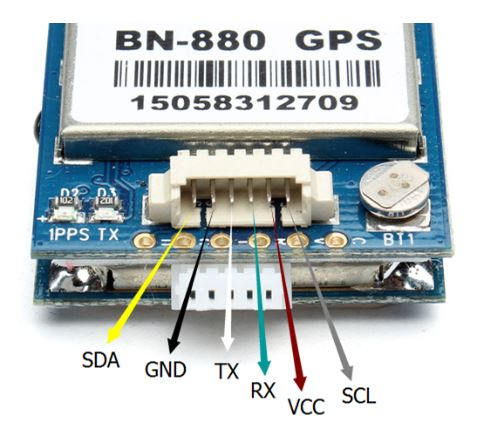
\includegraphics[width=0.4\linewidth]{figuras/BN-880-pinout.jpg}
    \caption{Módulo \gls{gps} BN-880 utilizado no protótipo e respetivo \emph{pinout}}
    \label{fig:gps}
\end{figure}

O módulo \gls{gps} disponibiliza os dados em formato \gls{nmea} \cite{nmea}, um padrão amplamente adotado para a transmissão de coordenadas de latitude, longitude, velocidade e tempo. Estes dados são enviados através de uma interface série \gls{uart}, que estabelece comunicação direta entre o módulo e o microcontrolador.  

No entanto, dado que a porta série principal do \gls{esp32} foi reservada para tarefas de \emph{debug} e monitorização via USB, recorreu-se a um conversor \gls{i2c}-\gls{uart} (SC16IS750), que permitiu a criação de uma porta série adicional a partir do barramento \gls{i2c}. Esta solução garantiu a integração do \gls{gps} sem comprometer a disponibilidade da interface série nativa do \gls{esp32}, mantendo a arquitetura modular e expansível do sistema.  

Um aspeto crítico na integração deste módulo prende-se com a compatibilidade elétrica. Embora o BN-880 seja alimentado a 5 V, o \gls{esp32} opera a 3.3 V nos seus pinos de entrada/saída digitais. Para evitar danos no microcontrolador e assegurar a comunicação fiável, foi introduzido um conversor de nível lógico, responsável por adaptar os sinais da interface \gls{uart} entre os dois dispositivos.  

A alimentação do módulo é assegurada diretamente pela linha de 5 V do sistema, enquanto as ligações de dados (TX e RX) passam pelo conversor de nível lógico antes de chegar ao \gls{esp32}. Esta configuração garante a integridade do sinal e a proteção dos módulos. As ligações elétricas detalhadas podem ser observadas no Anexo \ref{anexo:pcb}, na Figura \ref{fig:esquematica-gps}, que apresenta a esquemática correspondente.  

Tal como o \gls{imu}, o módulo \gls{gps} foi instalado no interior da caixa estanque, com especial atenção à orientação da antena integrada, de forma a manter visibilidade direta com o céu e reduzir obstruções ao sinal.

\subsection{Comunicação}

A comunicação entre o \gls{usv} e a estação remota é assegurada pela tecnologia \acrfull{lora}, integrada no próprio \gls{esp32} TTGO \gls{lora}32, que incorpora o transceptor Semtech SX1276. Esta solução permitiu simplificar a arquitetura de \emph{\emph{hardware}}, eliminando a necessidade de módulos externos dedicados de rádio e garantindo ao mesmo tempo baixo consumo energético e elevada robustez em cenários de operação remota.  

A configuração do transceptor \gls{lora} foi realizada de acordo com a regulamentação europeia, utilizando uma frequência de operação de 866 MHz. 

O sistema foi configurado para operar com um \emph{Spreading Factor} de 12, que maximiza o alcance da comunicação ao custo de um \emph{bitrate} mais baixo. Apesar de não ter sido modificada no protótipo, a biblioteca \gls{lora} permite também ajustar parâmetros como a potência de transmissão, a largura de banda e o esquema de codificação, o que poderá ser explorado em trabalhos futuros para otimizar o compromisso entre alcance, robustez e eficiência energética.  

A comunicação pode ser utilizada para dois propósitos principais:  

\begin{enumerate}
    \item Comandos remotos, que foram implementados no âmbito deste trabalho, consistem na receção de instruções provenientes da estação remota. Estes comandos permitem tanto a atualização de rotas sob a forma de \emph{waypoints} como a navegação manual, através de ordens de movimento direto (avante e atrás), lateral (esquerda e direita) e paragem. A implementação destes comandos garante a possibilidade de alternar entre controlo autónomo e intervenção manual sempre que necessário.  
    \item Telemetria, que consiste no envio periódico de dados essenciais para a monitorização do sistema, incluindo posição \gls{gps}, orientação obtida pelo \gls{imu}, estado da bateria e modo de controlo ativo (manual ou automático). Esta funcionalidade não foi implementada na presente fase do trabalho, encontrando-se prevista para desenvolvimentos futuros.  
\end{enumerate}

\subsection{\acrfull{pcb}}
\label{subsec:pcb}

Com o objetivo de integrar todos os módulos do sistema de forma compacta e fiável, foi desenvolvida uma \gls{pcb} dedicada, que reúne numa única placa todos os elementos de controlo, aquisição e comunicação do protótipo do \gls{usv}. A centralização numa única \gls{pcb} reduz significativamente a complexidade da cablagem, minimiza possíveis falhas de ligação e facilita a montagem, manutenção e escalabilidade do sistema.  

Na sua conceção, a placa incorpora diferentes blocos funcionais. O processamento central é assegurado pelo módulo TTGO \gls{lora}32, baseado no microcontrolador \gls{esp32}, que tem a responsabilidade de gerar sinais \gls{pwm}, gerir a comunicação via \gls{i2c}, \gls{uart} e \gls{lora}, e garantir a ligação ao sistema através de uma antena dedicada. O controlo dos motores é realizado por um expansor PCA9685, que disponibiliza até 16 canais de \gls{pwm}, dos quais dois foram configurados para comandar os propulsores através dos respetivos \gls{esc}.  

No que respeita à navegação, o recetor \gls{gps} BN-880 foi integrado no sistema através de um conversor SC16IS750, que atua como ponte entre a interface \gls{uart} do módulo e o barramento \gls{i2c}, permitindo a sua comunicação com o microcontrolador sem comprometer a arquitetura modular. Complementarmente, o sensor \gls{imu} ICM-20948, também conectado por \gls{i2c}, assegura medições contínuas de aceleração, velocidade angular e intensidade do campo magnético nos três eixos, fundamentais para a estimativa da orientação do veículo.  

Por fim, a gestão de energia foi contemplada através da inclusão de conectores específicos para a entrada de energia principal a 12~V, interruptores de corte que permitem desligar o sistema de forma segura e \gls{led} indicadores que fornecem feedback visual sobre o estado de funcionamento.  

A Figura \ref{fig:pcb-esquematica-vs-real} ilustra a comparação entre a esquemática desenvolvida e a implementação física da placa.

\begin{figure}[H]
    \centering
    \begin{minipage}{0.45\linewidth}
        \centering
        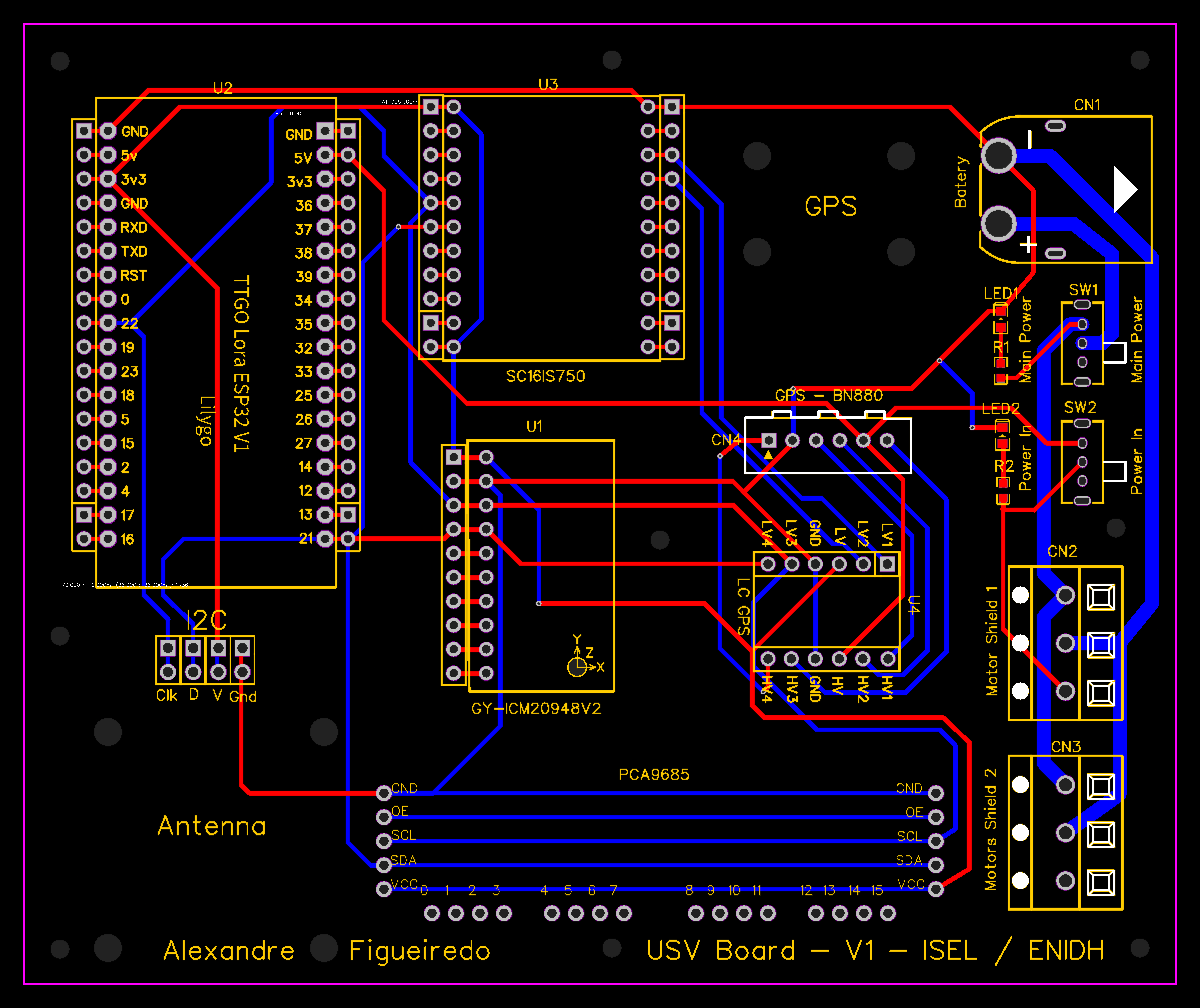
\includegraphics[width=0.80\linewidth]{figuras/PCB_PCB_USV-Board_2025-09-21.png}
        \caption*{(A) \emph{Layout} da PCB}
    \end{minipage}
    \hfill
    \begin{minipage}{0.40\linewidth}
        \centering
        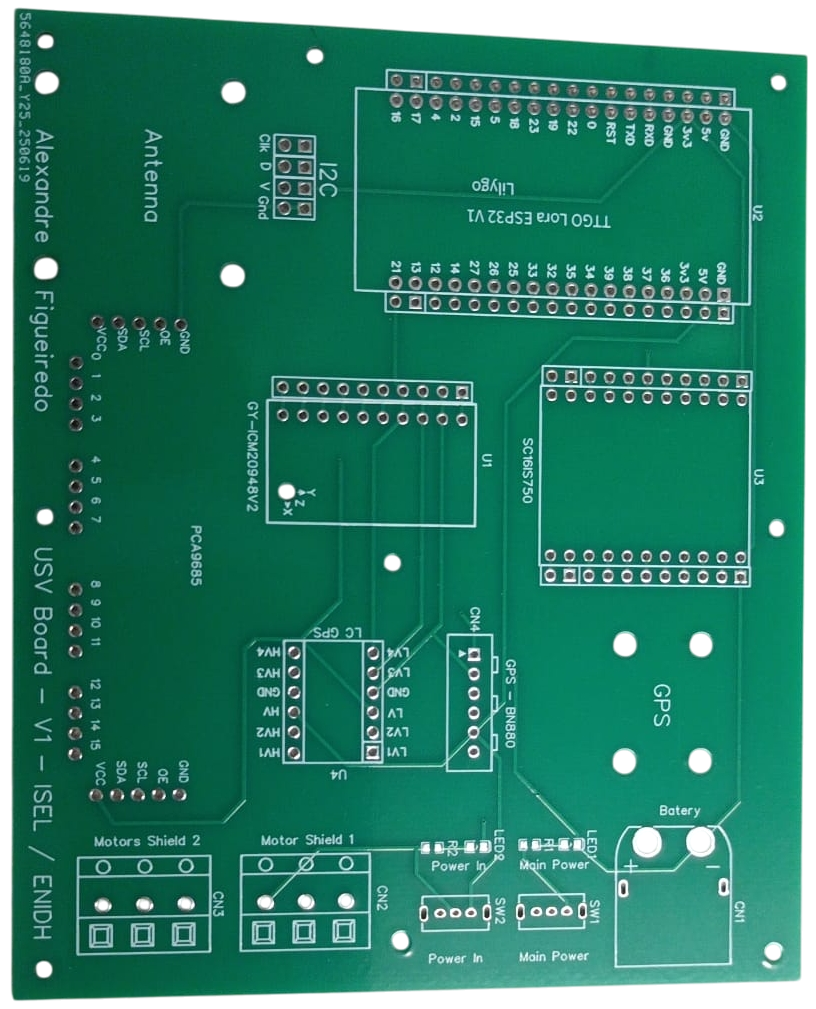
\includegraphics[width=0.80\linewidth,angle=90]{figuras/pcb-real.png}
        \caption*{(B) Implementação real}
    \end{minipage}
    \caption{Comparação entre a esquemática (A) e a implementação física (B) da \gls{pcb}}
    \label{fig:pcb-esquematica-vs-real}
\end{figure}

As esquemáticas completas encontram-se documentadas no Anexo \ref{anexo:pcb}, permitindo uma análise detalhada de cada ligação elétrica. A versão montada da \gls{pcb} encontra-se representada na Figura \ref{fig:pcb-final}, onde é possível identificar a disposição dos principais módulos e as camadas de interligação.  

\begin{figure}[H]
    \centering
    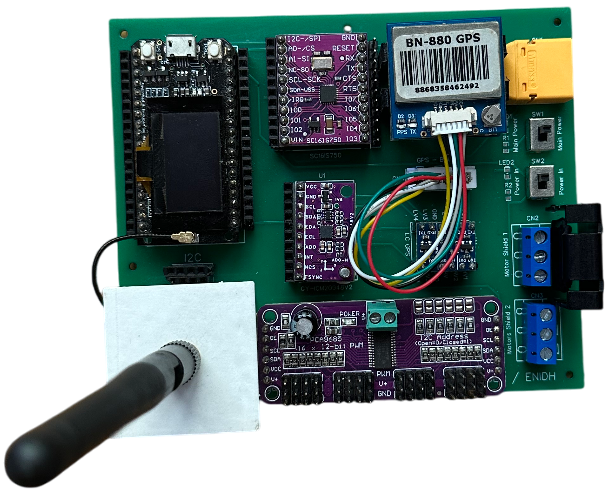
\includegraphics[width=0.5\linewidth]{figuras/pcb-final.png}
    \caption{Versão montada da \gls{pcb} desenvolvida para o protótipo do \gls{usv}}
    \label{fig:pcb-final}
\end{figure}

Em suma, a integração de todos os módulos numa única \gls{pcb} permitiu não só simplificar o design global do sistema, mas também garantir maior fiabilidade elétrica e reduzir a probabilidade de falhas por mau contacto ou cablagem incorreta. Esta abordagem aumenta a robustez do protótipo e facilita a sua replicação em versões futuras.

\section{Implementação de \emph{Software}}
\label{sec:implementacao-software}

A implementação de \emph{software} constituiu a camada lógica do sistema desenvolvido, responsável por coordenar a interação entre os diferentes módulos de \emph{\emph{hardware}}, assegurar o processamento em tempo real dos dados de sensores, gerir a comunicação sem fios e aplicar os algoritmos de navegação. Esta camada foi concebida de forma modular, permitindo que cada componente seja desenvolvido, testado e substituído de forma independente, sem comprometer a integridade do sistema global.  

O código foi estruturado para garantir três requisitos principais: funcionamento não bloqueante, escalabilidade e reutilização. O primeiro requisito assegura que todas as tarefas críticas, como leitura de sensores, controlo dos motores e receção de comandos, são executadas sem interrupções prolongadas, preservando a responsividade do sistema. O segundo requisito garante que novos módulos ou algoritmos de controlo podem ser facilmente integrados, acompanhando a evolução do protótipo. O terceiro requisito promove a portabilidade do código para outros projetos semelhantes, mantendo a mesma filosofia modular que guiou a implementação do Robot Didático \cite{didactic-robot-thesis}.  

Importa ainda destacar que todo o código desenvolvido no âmbito desta \gls{tfm} foi disponibilizado em regime de \emph{open source}, encontrando-se acessível num repositório público de controlo de versões na plataforma GitHub \cite{github-usv}. Esta decisão assegura não apenas a transparência e reprodutibilidade científica, mas também a possibilidade de reutilização, extensão e validação por parte de outros estudantes, investigadores, profissionais da área e qualquer curioso.

Ao longo desta secção são descritos os principais aspetos da implementação de \emph{software}, incluindo a integração dos subsistemas no ciclo principal na Subsecção~\ref{sec:integracao}, a arquitetura modular do código na Subsecção~\ref{subsec:arquitetura-codigo}, o controlo dos motores na Subsecção~\ref{subsec:controlo-de-motores}, a leitura e processamento dos sensores na Subsecção~\ref{subsec:processamento-sensores} e a comunicação via \gls{lora} com mensagens estruturadas em \emph{Protobuf} na Subsecção~\ref{subsec:comunicacao-lora}. Estes elementos, em conjunto, constituem a base funcional que permite ao veículo operar de forma autónoma ou manual, com monitorização e controlo em tempo real.

\subsection{Integração do Sistema}
\label{sec:integracao}

A integração do sistema foi concebida de forma modular, com o objetivo de simplificar o desenvolvimento e permitir que novos utilizadores ou projetos derivados possam reutilizar o código com um esforço mínimo. A interface de utilização resume-se à inicialização do objeto principal \texttt{\gls{usv}} e à execução do método \texttt{loop()}, que coordena todos os subsistemas. Os sensores disponibilizam métodos dedicados para aceder aos dados mais recentes (e.g. \texttt{getGPSData()}, \texttt{getIMUData()}), garantindo uma utilização intuitiva e não bloqueante.  

\subsubsection{Estrutura do Código Principal}

O código principal (contido no ficheiro \texttt{main\_usv.cpp}) organiza-se em duas funções fundamentais: \texttt{setup()}, responsável pela inicialização de todos os módulos (sensores, comunicação, propulsores e controladores), e \texttt{loop()}, que executa repetidamente o ciclo de controlo. A execução do \texttt{loop()} do objeto \texttt{\gls{usv}} é suficiente para garantir a atualização contínua de sensores, o envio de telemetria, a receção de comandos e o controlo dos motores. A lógica interna foi desenhada para operar de forma assíncrona, evitando chamadas bloqueantes que pudessem comprometer a responsividade do sistema. 

A Listagem \ref{lst:main-usv-cpp} apresenta o código completo do ficheiro \texttt{main\_usv.cpp}, ilustrando a simplicidade da interface de controlo.

\lstinputlisting[caption=Estrutura principal do programa do \gls{usv}, label={lst:main-usv-cpp}, style=BetterCPP]{code/minimal/main_usv.cpp}

É importante destacar que os dados provenientes do \gls{gps} e da \gls{imu} são processados de forma independente. A obtenção destas informações é realizada explicitamente através das chamadas aos métodos \texttt{getGPSData()} e \texttt{getIMUData()}, nas linhas 27 e 28 do código, respetivamente. Esta abordagem reflete uma decisão arquitetural relevante, pois garante que o objeto \texttt{USV} não está rigidamente acoplado a implementações específicas de sensores, mas antes a interfaces genéricas que fornecem dados estruturados de posicionamento e orientação.  

Desta forma, a substituição ou atualização de sensores pode ser efetuada sem necessidade de alterar a lógica central do sistema, preservando a modularidade e a escalabilidade do \emph{software}. A profundidade desta estratégia de abstração e independência sensorial é analisada em maior detalhe na Subsecção~\ref{subsec:processamento-sensores}, onde se descrevem os mecanismos de aquisição e processamento de dados dos sensores.

\subsubsection{Sincronização de Sensores, Motores e Comunicação}  

A atualização dos sensores é realizada periodicamente, com cada módulo a gerir internamente a sua própria leitura. O \gls{gps}, através da classe \texttt{GPS\_BN880}, descodifica continuamente as mensagens \gls{nmea} recebidas via ponte \gls{i2c}-\gls{uart}, enquanto o \gls{imu} (\texttt{IMU\_ICM\_20948}) atualiza os valores de aceleração, rotação e orientação utilizando o filtro de Madgwick \cite{madgwick-filter}. Os propulsores são controlados via \gls{pwm} gerado pelo expansor, com os valores definidos pela lógica de navegação implementada na classe \texttt{Control}. Paralelamente, a comunicação \gls{lora}, encapsulada nas classes \texttt{LoRaDuplex} e \texttt{LoRaProto}, trata de forma não bloqueante tanto o envio periódico de telemetria como a receção de pacotes de controlo. Esta abordagem garante que nenhum módulo interrompe a execução do ciclo principal, assegurando a fluidez da operação em tempo real.

\subsubsection{Testes Incrementais}

A validação do sistema foi realizada de forma incremental, seguindo uma estratégia de integração progressiva. Numa primeira fase foram testados os motores de forma isolada, validando a geração de sinais \gls{pwm}, o processo de armamento dos \gls{esc} e a resposta dos propulsores. Posteriormente, os sensores foram integrados individualmente, confirmando a calibração do \gls{imu} e a receção estável de coordenadas \gls{gps}. Numa fase seguinte, foi estabelecida a comunicação via \gls{lora}, assegurando a transmissão de telemetria e a receção de comandos em tempo real. Finalmente, todos os módulos foram integrados no sistema completo, testando a coerência do funcionamento conjunto, incluindo a execução de rotas automáticas baseadas em \emph{waypoints} e a alternância entre modos manual e automático.

Em síntese, a arquitetura de \emph{software} foi desenhada para ser modular, escalável e de fácil utilização, permitindo que qualquer utilizador possa controlar o \gls{usv} com apenas algumas chamadas de alto nível, enquanto a lógica interna garante a sincronização e integração de todos os subsistemas de forma transparente.

\subsection{Arquitetura do Código}
\label{subsec:arquitetura-codigo}

A arquitetura de \emph{software} foi concebida de forma modular, seguindo princípios de encapsulamento e separação de responsabilidades. Cada componente do sistema foi implementado numa biblioteca própria, organizada em \emph{packages} correspondentes às suas funções principais, como propulsão, sensores, comunicação e controlo. Esta abordagem modular facilita a manutenção, promove a reutilização do código e assegura a escalabilidade do sistema, permitindo que novos sensores ou atuadores possam ser integrados com alterações mínimas à base existente.  

A Figura~\ref{fig:uml-simplificado} apresenta um diagrama \gls{uml} simplificado que ilustra a arquitetura do sistema e as interações entre as suas classes principais (para diagramas mais complexos ver Anexo \ref{anexo:diagramas-de-classes}). 

\begin{figure}[H]
  \centering
  \resizebox{\textwidth}{!}{%
    % generated by Plantuml 1.2024.3       
\definecolor{plantucolor0000}{RGB}{255,255,255}
\definecolor{plantucolor0001}{RGB}{0,0,0}
\definecolor{plantucolor0002}{RGB}{238,238,238}
\definecolor{plantucolor0003}{RGB}{221,221,221}
\definecolor{plantucolor0004}{RGB}{204,204,204}
\definecolor{plantucolor0005}{RGB}{187,187,187}
\begin{tikzpicture}[yscale=-1
,pstyle0/.style={color=black,fill=white,line width=1.0pt}
,pstyle1/.style={color=black,line width=1.0pt}
,pstyle6/.style={color=black,fill=black,line width=1.0pt}
]
\draw[pstyle0] (794.5pt,11.602pt) -- (917.9187pt,11.602pt) arc(270:360:3.75pt)  -- (927.4187pt,36.6699pt) -- (974.5pt,36.6699pt) arc(270:360:2.5pt)  -- (977pt,349.102pt) arc(0:90:2.5pt)  -- (794.5pt,351.602pt) arc(90:180:2.5pt)  -- (792pt,14.102pt) arc(180:270:2.5pt) ;
\draw[pstyle1] (792pt,36.6699pt) -- (927.4187pt,36.6699pt);
\node at (796pt,13.602pt)[below right,color=black]{\textbf{Robot Didático}};
\draw[color=black,fill=plantucolor0002,line width=1.0pt] (13.5pt,19.602pt) -- (47.6714pt,19.602pt) arc(270:360:3.75pt)  -- (57.1714pt,44.6699pt) -- (761.5pt,44.6699pt) arc(270:360:2.5pt)  -- (764pt,117.102pt) arc(0:90:2.5pt)  -- (13.5pt,119.602pt) arc(90:180:2.5pt)  -- (11pt,22.102pt) arc(180:270:2.5pt) ;
\draw[pstyle1] (11pt,44.6699pt) -- (57.1714pt,44.6699pt);
\node at (15pt,21.602pt)[below right,color=black]{\textbf{USV}};
\draw[color=black,fill=plantucolor0003,line width=1.0pt] (404.5pt,340.602pt) -- (468.9667pt,340.602pt) arc(270:360:3.75pt)  -- (478.4667pt,365.6699pt) -- (531.5pt,365.6699pt) arc(270:360:2.5pt)  -- (534pt,473.102pt) arc(0:90:2.5pt)  -- (404.5pt,475.602pt) arc(90:180:2.5pt)  -- (402pt,343.102pt) arc(180:270:2.5pt) ;
\draw[pstyle1] (402pt,365.6699pt) -- (478.4667pt,365.6699pt);
\node at (406pt,342.602pt)[below right,color=black]{\textbf{Control}};
\draw[color=black,fill=plantucolor0004,line width=1.0pt] (601pt,428.602pt) -- (665.6727pt,428.602pt) arc(270:360:3.75pt)  -- (675.1727pt,453.6699pt) -- (722pt,453.6699pt) arc(270:360:2.5pt)  -- (724.5pt,606.102pt) arc(0:90:2.5pt)  -- (601pt,608.602pt) arc(90:180:2.5pt)  -- (598.5pt,431.102pt) arc(180:270:2.5pt) ;
\draw[pstyle1] (598.5pt,453.6699pt) -- (675.1727pt,453.6699pt);
\node at (602.5pt,430.602pt)[below right,color=black]{\textbf{Sensors}};
\draw[color=black,fill=plantucolor0005,line width=1.0pt] (181pt,303.602pt) -- (315.2991pt,303.602pt) arc(270:360:3.75pt)  -- (324.7991pt,328.6699pt) -- (325pt,328.6699pt) arc(270:360:2.5pt)  -- (327.5pt,481.102pt) arc(0:90:2.5pt)  -- (181pt,483.602pt) arc(90:180:2.5pt)  -- (178.5pt,306.102pt) arc(180:270:2.5pt) ;
\draw[pstyle1] (178.5pt,328.6699pt) -- (324.7991pt,328.6699pt);
\node at (182.5pt,305.602pt)[below right,color=black]{\textbf{Communication}};
\draw[pstyle0] (848.5pt,295.102pt) arc (180:270:5pt) -- (853.5pt,290.102pt) -- (915.8897pt,290.102pt) arc (270:360:5pt) -- (920.8897pt,295.102pt) -- (920.8897pt,330.1699pt) arc (0:90:5pt) -- (915.8897pt,335.1699pt) -- (853.5pt,335.1699pt) arc (90:180:5pt) -- (848.5pt,330.1699pt) -- cycle;
\draw[pstyle0] (860.5pt,304.6359pt) ellipse (8pt and 8pt);
\node at (860.5pt,304.6359pt)[]{\textbf{\Large C}};
\node at (871.5pt,295.102pt)[below right,color=black]{Robot};
\draw[pstyle1] (849.5pt,319.1699pt) -- (919.8897pt,319.1699pt);
\draw[pstyle1] (849.5pt,327.1699pt) -- (919.8897pt,327.1699pt);
\draw[pstyle0] (830.5pt,215.102pt) arc (180:270:5pt) -- (835.5pt,210.102pt) -- (933.7857pt,210.102pt) arc (270:360:5pt) -- (938.7857pt,215.102pt) -- (938.7857pt,250.1699pt) arc (0:90:5pt) -- (933.7857pt,255.1699pt) -- (835.5pt,255.1699pt) arc (90:180:5pt) -- (830.5pt,250.1699pt) -- cycle;
\draw[pstyle0] (842.5pt,224.6359pt) ellipse (8pt and 8pt);
\node at (842.5pt,224.6359pt)[]{\textbf{\Large C}};
\node at (853.5pt,215.102pt)[below right,color=black]{Movement};
\draw[pstyle1] (831.5pt,239.1699pt) -- (937.7857pt,239.1699pt);
\draw[pstyle1] (831.5pt,247.1699pt) -- (937.7857pt,247.1699pt);
\draw[pstyle0] (847.5pt,135.102pt) arc (180:270:5pt) -- (852.5pt,130.102pt) -- (916.7244pt,130.102pt) arc (270:360:5pt) -- (921.7244pt,135.102pt) -- (921.7244pt,170.1699pt) arc (0:90:5pt) -- (916.7244pt,175.1699pt) -- (852.5pt,175.1699pt) arc (90:180:5pt) -- (847.5pt,170.1699pt) -- cycle;
\draw[pstyle0] (859.5pt,144.6359pt) ellipse (8pt and 8pt);
\node at (859.5pt,144.6359pt)[]{\textbf{\Large C}};
\node at (870.5pt,135.102pt)[below right,color=black]{Motor};
\draw[pstyle1] (848.5pt,159.1699pt) -- (920.7244pt,159.1699pt);
\draw[pstyle1] (848.5pt,167.1699pt) -- (920.7244pt,167.1699pt);
\draw[pstyle0] (808pt,55.102pt) arc (180:270:5pt) -- (813pt,50.102pt) -- (956.4972pt,50.102pt) arc (270:360:5pt) -- (961.4972pt,55.102pt) -- (961.4972pt,90.1699pt) arc (0:90:5pt) -- (956.4972pt,95.1699pt) -- (813pt,95.1699pt) arc (90:180:5pt) -- (808pt,90.1699pt) -- cycle;
\draw[pstyle0] (820pt,64.6359pt) ellipse (8pt and 8pt);
\node at (820pt,64.6359pt)[]{\textbf{\Large C}};
\node at (831pt,55.102pt)[below right,color=black]{MotorController};
\draw[pstyle1] (809pt,79.1699pt) -- (960.4972pt,79.1699pt);
\draw[pstyle1] (809pt,87.1699pt) -- (960.4972pt,87.1699pt);
\draw[pstyle0] (27pt,63.102pt) arc (180:270:5pt) -- (32pt,58.102pt) -- (79.2148pt,58.102pt) arc (270:360:5pt) -- (84.2148pt,63.102pt) -- (84.2148pt,98.1699pt) arc (0:90:5pt) -- (79.2148pt,103.1699pt) -- (32pt,103.1699pt) arc (90:180:5pt) -- (27pt,98.1699pt) -- cycle;
\draw[pstyle0] (39pt,72.6359pt) ellipse (8pt and 8pt);
\node at (39pt,72.6359pt)[]{\textbf{\Large C}};
\node at (50pt,63.102pt)[below right,color=black]{USV};
\draw[pstyle1] (28pt,87.1699pt) -- (83.2148pt,87.1699pt);
\draw[pstyle1] (28pt,95.1699pt) -- (83.2148pt,95.1699pt);
\draw[pstyle0] (144pt,63.102pt) arc (180:270:5pt) -- (149pt,58.102pt) -- (355.9463pt,58.102pt) arc (270:360:5pt) -- (360.9463pt,63.102pt) -- (360.9463pt,98.1699pt) arc (0:90:5pt) -- (355.9463pt,103.1699pt) -- (149pt,103.1699pt) arc (90:180:5pt) -- (144pt,98.1699pt) -- cycle;
\draw[pstyle0] (156pt,72.6359pt) ellipse (8pt and 8pt);
\node at (156pt,72.6359pt)[]{\textbf{\Large C}};
\node at (167pt,63.102pt)[below right,color=black]{MovementTwoThrusters};
\draw[pstyle1] (145pt,87.1699pt) -- (359.9463pt,87.1699pt);
\draw[pstyle1] (145pt,95.1699pt) -- (359.9463pt,95.1699pt);
\draw[pstyle0] (421pt,63.102pt) arc (180:270:5pt) -- (426pt,58.102pt) -- (509.7492pt,58.102pt) arc (270:360:5pt) -- (514.7492pt,63.102pt) -- (514.7492pt,98.1699pt) arc (0:90:5pt) -- (509.7492pt,103.1699pt) -- (426pt,103.1699pt) arc (90:180:5pt) -- (421pt,98.1699pt) -- cycle;
\draw[pstyle0] (433pt,72.6359pt) ellipse (8pt and 8pt);
\node at (433pt,72.6359pt)[]{\textbf{\Large C}};
\node at (444pt,63.102pt)[below right,color=black]{Thruster};
\draw[pstyle1] (422pt,87.1699pt) -- (513.7492pt,87.1699pt);
\draw[pstyle1] (422pt,95.1699pt) -- (513.7492pt,95.1699pt);
\draw[pstyle0] (575pt,63.102pt) arc (180:270:5pt) -- (580pt,58.102pt) -- (743.0142pt,58.102pt) arc (270:360:5pt) -- (748.0142pt,63.102pt) -- (748.0142pt,98.1699pt) arc (0:90:5pt) -- (743.0142pt,103.1699pt) -- (580pt,103.1699pt) arc (90:180:5pt) -- (575pt,98.1699pt) -- cycle;
\draw[pstyle0] (587pt,72.6359pt) ellipse (8pt and 8pt);
\node at (587pt,72.6359pt)[]{\textbf{\Large S}};
\node at (598pt,63.102pt)[below right,color=black]{ThrusterController};
\draw[pstyle1] (576pt,87.1699pt) -- (747.0142pt,87.1699pt);
\draw[pstyle1] (576pt,95.1699pt) -- (747.0142pt,95.1699pt);
\draw[pstyle0] (426pt,392.102pt) arc (180:270:5pt) -- (431pt,387.102pt) -- (505.32pt,387.102pt) arc (270:360:5pt) -- (510.32pt,392.102pt) -- (510.32pt,427.1699pt) arc (0:90:5pt) -- (505.32pt,432.1699pt) -- (431pt,432.1699pt) arc (90:180:5pt) -- (426pt,427.1699pt) -- cycle;
\draw[pstyle0] (438pt,401.6359pt) ellipse (8pt and 8pt);
\node at (438pt,401.6359pt)[]{\textbf{\Large C}};
\node at (449pt,392.102pt)[below right,color=black]{Control};
\draw[pstyle1] (427pt,416.1699pt) -- (509.32pt,416.1699pt);
\draw[pstyle1] (427pt,424.1699pt) -- (509.32pt,424.1699pt);
\draw[pstyle0] (615.5pt,472.102pt) arc (180:270:5pt) -- (620.5pt,467.102pt) -- (702.093pt,467.102pt) arc (270:360:5pt) -- (707.093pt,472.102pt) -- (707.093pt,507.1699pt) arc (0:90:5pt) -- (702.093pt,512.1699pt) -- (620.5pt,512.1699pt) arc (90:180:5pt) -- (615.5pt,507.1699pt) -- cycle;
\draw[pstyle0] (627.5pt,481.6359pt) ellipse (8pt and 8pt);
\node at (627.5pt,481.6359pt)[]{\textbf{\Large C}};
\node at (638.5pt,472.102pt)[below right,color=black]{GPSData};
\draw[pstyle1] (616.5pt,496.1699pt) -- (706.093pt,496.1699pt);
\draw[pstyle1] (616.5pt,504.1699pt) -- (706.093pt,504.1699pt);
\draw[pstyle0] (614.5pt,552.102pt) arc (180:270:5pt) -- (619.5pt,547.102pt) -- (703.2492pt,547.102pt) arc (270:360:5pt) -- (708.2492pt,552.102pt) -- (708.2492pt,587.1699pt) arc (0:90:5pt) -- (703.2492pt,592.1699pt) -- (619.5pt,592.1699pt) arc (90:180:5pt) -- (614.5pt,587.1699pt) -- cycle;
\draw[pstyle0] (626.5pt,561.6359pt) ellipse (8pt and 8pt);
\node at (626.5pt,561.6359pt)[]{\textbf{\Large C}};
\node at (637.5pt,552.102pt)[below right,color=black]{IMUData};
\draw[pstyle1] (615.5pt,576.1699pt) -- (707.2492pt,576.1699pt);
\draw[pstyle1] (615.5pt,584.1699pt) -- (707.2492pt,584.1699pt);
\draw[pstyle0] (225pt,347.102pt) arc (180:270:5pt) -- (230pt,342.102pt) -- (275.04pt,342.102pt) arc (270:360:5pt) -- (280.04pt,347.102pt) -- (280.04pt,382.1699pt) arc (0:90:5pt) -- (275.04pt,387.1699pt) -- (230pt,387.1699pt) arc (90:180:5pt) -- (225pt,382.1699pt) -- cycle;
\draw[pstyle0] (237pt,356.6359pt) ellipse (8pt and 8pt);
\node at (237pt,356.6359pt)[]{\textbf{\Large C}};
\node at (248pt,347.102pt)[below right,color=black]{Led};
\draw[pstyle1] (226pt,371.1699pt) -- (279.04pt,371.1699pt);
\draw[pstyle1] (226pt,379.1699pt) -- (279.04pt,379.1699pt);
\draw[pstyle0] (219.5pt,427.102pt) arc (180:270:5pt) -- (224.5pt,422.102pt) -- (280.3588pt,422.102pt) arc (270:360:5pt) -- (285.3588pt,427.102pt) -- (285.3588pt,462.1699pt) arc (0:90:5pt) -- (280.3588pt,467.1699pt) -- (224.5pt,467.1699pt) arc (90:180:5pt) -- (219.5pt,462.1699pt) -- cycle;
\draw[pstyle0] (231.5pt,436.6359pt) ellipse (8pt and 8pt);
\node at (231.5pt,436.6359pt)[]{\textbf{\Large C}};
\node at (242.5pt,427.102pt)[below right,color=black]{LoRa};
\draw[pstyle1] (220.5pt,451.1699pt) -- (284.3588pt,451.1699pt);
\draw[pstyle1] (220.5pt,459.1699pt) -- (284.3588pt,459.1699pt);
\draw[pstyle1] (76pt,103.272pt) ..controls (76pt,161.642pt) and (76pt,312.602pt) .. (76pt,312.602pt) ..controls (76pt,312.602pt) and (673.56pt,312.602pt) .. (830.45pt,312.602pt);
\draw[pstyle1] (848.45pt,312.602pt) -- (830.45pt,306.602pt) -- (830.45pt,318.602pt) -- (848.45pt,312.602pt) -- cycle;
\draw[pstyle1] (324pt,103.362pt) ..controls (324pt,145.762pt) and (324pt,232.602pt) .. (324pt,232.602pt) ..controls (324pt,232.602pt) and (671.58pt,232.602pt) .. (812.25pt,232.602pt);
\draw[pstyle1] (830.25pt,232.602pt) -- (812.25pt,226.602pt) -- (812.25pt,238.602pt) -- (830.25pt,232.602pt) -- cycle;
\draw[pstyle1] (468pt,103.382pt) ..controls (468pt,124.482pt) and (468pt,152.602pt) .. (468pt,152.602pt) ..controls (468pt,152.602pt) and (726.94pt,152.602pt) .. (829.17pt,152.602pt);
\draw[pstyle1] (847.17pt,152.602pt) -- (829.17pt,146.602pt) -- (829.17pt,158.602pt) -- (847.17pt,152.602pt) -- cycle;
\draw[pstyle1] (748.04pt,76.602pt) ..controls (767.75pt,76.602pt) and (770.56pt,76.602pt) .. (789.82pt,76.602pt);
\draw[pstyle1] (807.82pt,76.602pt) -- (789.82pt,70.602pt) -- (789.82pt,82.602pt) -- (807.82pt,76.602pt) -- cycle;
\draw[pstyle1] (96.15pt,80.602pt) ..controls (112.37pt,80.602pt) and (121.79pt,80.602pt) .. (143.91pt,80.602pt);
\draw[pstyle1] (84.15pt,80.602pt) -- (90.15pt,84.602pt) -- (96.15pt,80.602pt) -- (90.15pt,76.602pt) -- (84.15pt,80.602pt) -- cycle;
\draw[pstyle1] (52pt,115.382pt) ..controls (52pt,198.392pt) and (52pt,467.852pt) .. (52pt,467.852pt) ..controls (52pt,467.852pt) and (152.775pt,467.852pt) .. (255.125pt,467.852pt) ..controls (306.3pt,467.852pt) and (357.8688pt,467.852pt) .. (397.4313pt,467.852pt) ..controls (398.6676pt,467.852pt) and (399.8922pt,467.852pt) .. (401.1047pt,467.852pt);
\draw[pstyle6] (52pt,103.382pt) -- (48pt,109.382pt) -- (52pt,115.382pt) -- (56pt,109.382pt) -- (52pt,103.382pt) -- cycle;
\draw[pstyle1] (60pt,115.372pt) ..controls (60pt,195.062pt) and (60pt,444.602pt) .. (60pt,444.602pt) ..controls (60pt,444.602pt) and (164.37pt,444.602pt) .. (219.41pt,444.602pt);
\draw[pstyle6] (60pt,103.372pt) -- (56pt,109.372pt) -- (60pt,115.372pt) -- (64pt,109.372pt) -- (60pt,103.372pt) -- cycle;
\draw[pstyle1] (68pt,115.362pt) ..controls (68pt,182.752pt) and (68pt,364.602pt) .. (68pt,364.602pt) ..controls (68pt,364.602pt) and (173.41pt,364.602pt) .. (224.88pt,364.602pt);
\draw[pstyle1] (68pt,103.362pt) -- (64pt,109.362pt) -- (68pt,115.362pt) -- (72pt,109.362pt) -- (68pt,103.362pt) -- cycle;
\draw[pstyle1] (44pt,103.212pt) ..controls (44pt,189.112pt) and (44pt,490.352pt) .. (44pt,490.352pt) ..controls (44pt,490.352pt) and (465.98pt,490.352pt) .. (609.34pt,490.352pt);
\draw[pstyle6] (615.34pt,490.352pt) -- (606.34pt,486.352pt) -- (610.34pt,490.352pt) -- (606.34pt,494.352pt) -- (615.34pt,490.352pt) -- cycle;
\draw[pstyle1] (36pt,103.222pt) ..controls (36pt,200.352pt) and (36pt,577.102pt) .. (36pt,577.102pt) ..controls (36pt,577.102pt) and (463.02pt,577.102pt) .. (608.49pt,577.102pt);
\draw[pstyle6] (614.49pt,577.102pt) -- (605.49pt,573.102pt) -- (609.49pt,577.102pt) -- (605.49pt,581.102pt) -- (614.49pt,577.102pt) -- cycle;
\draw[pstyle1] (534.674pt,467.852pt) ..controls (534.9091pt,467.852pt) and (535.1444pt,467.852pt) .. (535.3801pt,467.852pt) ..controls (539.1499pt,467.852pt) and (542.9855pt,467.852pt) .. (546.8607pt,467.852pt) ..controls (554.6111pt,467.852pt) and (562.5202pt,467.852pt) .. (570.3795pt,467.852pt) ..controls (586.0981pt,467.852pt) and (595.6175pt,467.852pt) .. (609.27pt,467.852pt);
\draw[pstyle6] (615.27pt,467.852pt) -- (606.27pt,463.852pt) -- (610.27pt,467.852pt) -- (606.27pt,471.852pt) -- (615.27pt,467.852pt) -- cycle;
\draw[pstyle1] (468pt,475.7586pt) ..controls (468pt,476.1757pt) and (468pt,476.6062pt) .. (468pt,477.0494pt) ..controls (468pt,477.9359pt) and (468pt,478.8733pt) .. (468pt,479.8568pt) ..controls (468pt,481.8238pt) and (468pt,483.9748pt) .. (468pt,486.27pt) ..controls (468pt,495.4504pt) and (468pt,506.9364pt) .. (468pt,518.1707pt) ..controls (468pt,540.6395pt) and (468pt,562.102pt) .. (468pt,562.102pt) ..controls (468pt,562.102pt) and (550.88pt,562.102pt) .. (608.16pt,562.102pt);
\draw[pstyle6] (614.16pt,562.102pt) -- (605.16pt,558.102pt) -- (609.16pt,562.102pt) -- (605.16pt,566.102pt) -- (614.16pt,562.102pt) -- cycle;
\draw[pstyle1] (297.7pt,466.852pt) ..controls (327.45pt,466.852pt) and (360.0775pt,466.852pt) .. (397.73pt,466.852pt) ..controls (398.9066pt,466.852pt) and (400.0765pt,466.852pt) .. (401.2388pt,466.852pt);
\draw[pstyle1] (285.7pt,466.852pt) -- (291.7pt,470.852pt) -- (297.7pt,466.852pt) -- (291.7pt,462.852pt) -- (285.7pt,466.852pt) -- cycle;
\draw[pstyle1] (527.34pt,80.602pt) ..controls (545.24pt,80.602pt) and (554.22pt,80.602pt) .. (574.62pt,80.602pt);
\draw[pstyle6] (515.34pt,80.602pt) -- (521.34pt,84.602pt) -- (527.34pt,80.602pt) -- (521.34pt,76.602pt) -- (515.34pt,80.602pt) -- cycle;
\draw[pstyle1] (373.2pt,80.602pt) ..controls (394.22pt,80.602pt) and (403.2pt,80.602pt) .. (420.93pt,80.602pt);
\draw[pstyle6] (361.2pt,80.602pt) -- (367.2pt,84.602pt) -- (373.2pt,80.602pt) -- (367.2pt,76.602pt) -- (361.2pt,80.602pt) -- cycle;
\end{tikzpicture}
%
  }
  \caption{Arquitetura simplificada do sistema \gls{usv}}
  \label{fig:uml-simplificado}
\end{figure}

Tal como se pode observar, o desenvolvimento partiu da biblioteca \texttt{USV}, que estende o projeto do robot didático descrito em \cite{didactic-robot-thesis}. Esse robot foi concebido de forma a ser genérico e extensível, suportando diferentes tipos de robôs móveis, incluindo \gls{usv}. No presente trabalho, a classe \texttt{USV} herda de \texttt{Robot} e encapsula toda a lógica específica do protótipo, integrando a gestão dos propulsores, a leitura de sensores e os mecanismos de comunicação. A sua utilização é simplificada através de métodos de alto nível como \texttt{begin()}, responsável pela inicialização do \emph{hardware}, e \texttt{loop()}, que coordena de forma não bloqueante a atualização de todos os módulos.  

O controlo da propulsão é implementado pela classe \texttt{MovementTwoThrusters}, que herda de \texttt{Movement} e abstrai a complexidade da utilização de dois motores independentes. Esta classe fornece métodos como \texttt{left()} e \texttt{right()} que permitem executar manobras diferenciais sem necessidade de interação direta com os sinais \gls{pwm}. Cada propulsor é representado pela classe \texttt{Thruster}, que estende de \texttt{Motor} e disponibiliza métodos de controlo direto, como \texttt{front(speed)}, \texttt{back(speed)} e \texttt{stop()}. O comportamento de cada propulsor é parametrizado através da estrutura \texttt{ThrusterController}, que herda de \texttt{MotorController} e define parâmetros como os pinos de \gls{pwm}, os pulsos mínimos, máximos e neutros, bem como a frequência do sinal.  

No que respeita aos sensores, foram criados pacotes independentes para \gls{gps} e \gls{imu}. A arquitetura foi desenhada de forma a desacoplar a lógica de aquisição de dados da lógica de utilização, permitindo que qualquer sensor capaz de preencher as estruturas \texttt{GPSData} ou \texttt{IMUData} seja integrado sem modificações na camada de aplicação. Esta característica garante flexibilidade na substituição de sensores e assegura a compatibilidade futura com diferentes modelos de \emph{hardware}.  

A comunicação foi organizada no pacote \texttt{Communication}. A classe \texttt{LoRaDuplex} encapsula a interface direta com o transceptor \gls{lora} integrado no TTGO \gls{lora}32, implementando a lógica de envio e receção de pacotes em formato texto ou binário. Por cima desta camada foi desenvolvida a classe \texttt{LoRaProto}, responsável pela serialização e desserialização de mensagens com recurso a \emph{Protobuf} \cite{google-protobuf}. A utilização de \emph{Protobuf} permite definir de forma clara e estruturada os formatos de mensagem, ao mesmo tempo que reduz significativamente o tamanho dos pacotes transmitidos. Por exemplo, uma mensagem \texttt{StateMessage} representada em formato textual ocupa 33 bytes, enquanto a mesma mensagem em formato binário ocupa apenas 6 bytes, como ilustrado na Listagem~\ref{lst:comp}.

\begin{lstlisting}[style={BetterCPP},caption={Comparação entre representação textual e binária com \emph{Protobuf}},label={lst:comp}]
-- String (JSON-like):
{"state":"MANUAL","manual":"FORWARD"}
Tamanho: 33 bytes

-- Protobuf (binario):
08 01 12 02 08 01
Tamanho: 6 bytes
\end{lstlisting}

Em comunicações \gls{lora}, uma métrica crítica é o tempo no ar (\acrfull{toa}), que corresponde à duração de transmissão de um pacote. O \gls{toa} depende do tamanho da mensagem ($N_{\text{payload}}$), do fator de espalhamento (SF), da largura de banda (BW) e do código de correção de erros (CR). O cálculo é realizado em três etapas principais.  

Primeiro, calcula-se a duração de um símbolo ($T_{\text{sym}}$), que depende diretamente do fator de espalhamento e da largura de banda:

\begin{equation}
T_{\text{sym}} = \frac{2^{SF}}{BW}
\label{eq:toa1}
\end{equation}

A Equação~\ref{eq:toa1} mostra que o aumento do SF (maior robustez contra ruído) provoca símbolos mais longos, aumentando o tempo de transmissão. Em contrapartida, quanto maior for a largura de banda, menor será a duração de cada símbolo.  

De seguida, determina-se o número de símbolos necessários para transportar a carga útil ($N_{\text{payload}}$):

\begin{equation}
N_{\text{payload}} = 8 + \max \left( \left\lceil \frac{8 \cdot PL - 4 \cdot SF + 28 + 16 \cdot CRC - 20 \cdot H}{4 \cdot (SF - 2 \cdot DE)} \right\rceil \cdot (CR+4), 0 \right)
\label{eq:toa2}
\end{equation}

Na Equação~\ref{eq:toa2}, $PL$ representa o tamanho da carga útil (em bytes), $CRC$ indica se o mecanismo de verificação de erros está ativo, $H$ distingue entre cabeçalho implícito ou explícito e $DE$ refere-se à otimização para baixas taxas de dados. Este cálculo permite estimar quantos símbolos adicionais são necessários, para além da pré-codificação e redundância.  

Finalmente, obtém-se o tempo total de transmissão de um pacote ($T_{\text{packet}}$), somando a duração do preâmbulo ao número de símbolos da carga útil:

\begin{equation}
T_{\text{packet}} = \left( N_{\text{preamble}} + 4.25 + N_{\text{payload}} \right) \cdot T_{\text{sym}}
\label{eq:toa3}
\end{equation}

Na Equação~\ref{eq:toa3}, $N_{\text{preamble}}$ corresponde ao número de símbolos de sincronização enviados no início de cada transmissão, enquanto o fator $4.25$ resulta de um ajuste especificado pelo protocolo \gls{lora} \cite{ttn-lora-phy-format}. Multiplicando pela duração de cada símbolo, obtém-se o tempo efetivo que o pacote permanece no ar.  

Aplicando estas fórmulas ao exemplo descrito, com SF12, BW de 125 kHz e CR = 4/5, a transmissão de uma mensagem de 33 bytes apresenta um \gls{toa} aproximado de $1.81$ segundos. Já para uma mensagem de apenas 6 bytes, o valor reduz-se para $0.99$ segundos. Esta redução de aproximadamente 45\% traduz-se numa menor probabilidade de colisões, numa diminuição da taxa de erro de pacotes e num consumo energético inferior.  

Assim, ainda que o alcance teórico permaneça constante (pois depende apenas de SF, BW e CR), o alcance efetivo em cenários práticos é superior para mensagens mais curtas. Isto deve-se ao facto de pacotes mais compactos reduzirem a probabilidade de erros acumulados, a taxa de colisões e o tempo de ocupação do canal, contribuindo para uma comunicação mais robusta e eficiente.

Ainda no pacote de comunicação encontra-se a classe \texttt{Led}, que abstrai o controlo visual do sistema através de \gls{led} de estado. Esta classe disponibiliza métodos simples como \texttt{on()}, \texttt{off()} e \texttt{blink(duration, interval)}, sendo que o comportamento intermitente é implementado de forma não bloqueante mediante a chamada periódica do método \texttt{update()}.  

Finalmente, a lógica de navegação e controlo do veículo foi encapsulada no pacote \texttt{Control}. A classe \texttt{Control} é responsável por gerir a alternância entre o modo manual e o modo automático, utilizando os dados dos sensores e os comandos recebidos via comunicação para determinar as ações a aplicar nos propulsores. No modo manual, os comandos são traduzidos diretamente em ações sobre os motores. No modo automático, foi implementado um controlo simples baseado em lógica \emph{on/off}: sempre que o erro de rumo (\emph{bearing}) é positivo, o veículo corrige para a esquerda, e quando o erro é negativo, corrige para a direita. Apesar de simples, este método revelou-se eficaz para um protótipo de dois propulsores. No entanto, a arquitetura modular permite a substituição futura deste mecanismo por controladores mais avançados, como \acrfull{pid} ou \acrfull{lqr}, sem impacto significativo no restante sistema.  

A Listagem~\ref{lst:control} apresenta a implementação da lógica de controlo responsável pela alternância entre os modos automático e manual de navegação. 

\lstinputlisting[caption={Excerto da classe \texttt{Control} demonstrando a lógica automática de controlo},label={lst:control},style=BetterCPP]{code/minimal/control.cpp}

O método \texttt{control()} inicia verificando o estado atual do sistema. Quando este se encontra em modo automático, o \gls{led} correspondente é ativado e o \gls{led} manual é desligado, fornecendo assim um \emph{feedback} visual imediato ao operador. De forma análoga, quando o modo manual é selecionado, o \gls{led} manual é ligado e o \gls{led} automático é desligado. Esta alternância simples assegura que o estado de operação do veículo é sempre claramente indicado.  

No modo automático, o método \texttt{automaticControl()} verifica se todos os \emph{waypoints} definidos foram percorridos. Caso isso ocorra, o \gls{led} automático entra em modo intermitente e o movimento é interrompido, sinalizando o fim da missão. Caso contrário, é chamado o método \texttt{setCourse()}, que recebe como parâmetro o erro de rumo acumulado (\texttt{lastBearingError}) e executa a correção necessária.  

A lógica implementada em \texttt{setCourse()} baseia-se diretamente no sinal desse erro: valores positivos correspondem a desvios que requerem uma correção para a direita, valores negativos exigem correções para a esquerda e, no caso de o erro ser nulo, o movimento é interrompido com a chamada a \texttt{movement.stop()}. Trata-se, portanto, de um controlador simples do tipo \emph{on/off}, que se revelou eficaz para o seguimento de trajetórias definidas por \emph{waypoints}. Apesar de básico, este mecanismo é suficiente para o protótipo descrito nesta \gls{tfm}, mantendo no entanto a possibilidade de evolução para controladores mais sofisticados, como \gls{pid} ou \gls{lqr}, graças à natureza modular do código.  

Em síntese, a arquitetura de \emph{software} concebida garante robustez, clareza e expansibilidade, constituindo uma base sólida não apenas para o funcionamento do protótipo, mas também para evoluções futuras em sistemas mais complexos.

\subsection{Controlo dos Motores}
\label{subsec:controlo-de-motores}

Como discutido na Secção~\ref{sec:esc}, o controlo dos motores é efetuado através de um \gls{esc}, que requer sinais de \gls{pwm} com larguras de pulso específicas, expressas em microssegundos, e não apenas uma variação do \emph{duty cycle}. O intervalo típico situa-se entre 1000~\(\mu s\) e 2000~\(\mu s\), correspondendo respetivamente às rotações máximas nos sentidos inverso e direto, sendo 1500~\(\mu s\) o ponto neutro em que o motor permanece parado. Torna-se assim necessário mapear valores percentuais de velocidade para larguras de pulso compatíveis com o \gls{esc}.  

Para esse fim, a classe \texttt{Thruster} inclui o método \texttt{setDirection(clockwise)}, que define o sentido de rotação (horário ou anti-horário) e ajusta os limites mínimo, máximo e neutro do sinal \gls{pwm}. Com esta abstração, funções de mais alto nível, como \texttt{front(speed)} e \texttt{back(speed)}, permitem ao programador fornecer apenas uma percentagem de velocidade, sendo a conversão para o sinal em microssegundos tratada internamente.  

A ponte entre o domínio temporal, expresso em microssegundos, e o domínio do controlador PCA9685, expresso em \emph{ticks} de 12~bits, é assegurada pelo método \texttt{pulseToTicks(microseconds)}. A relação matemática implementada encontra-se expressa na Equação~\ref{eq:pulsetoticks}.  

\begin{equation}
n_{ticks} = \frac{t_{pulse} \cdot N_{ticks}}{10^6 / f_{PWM}}
\label{eq:pulsetoticks}
\end{equation}

em que \(t_{pulse}\) representa a largura de pulso em microssegundos, \(N_{ticks} = 4096\) é a resolução interna do PCA9685 em ticks e \(f_{PWM} = 20000\) a frequência de operação configurada em microssegundos. Esta conversão garante que os valores de pulso mínimo, máximo e neutro são corretamente interpretados pelo \gls{esc}.  

A Listagem~\ref{lst:thruster-cpp} apresenta parte da implementação da classe \texttt{Thruster}, ilustrando a lógica de mapeamento dos sinais \gls{pwm} para cada direção de rotação.  

\lstinputlisting[caption=Parte da classe \texttt{Thruster}, label={lst:thruster-cpp}, style=BetterCPP]{code/minimal/thruster.cpp}

Na função \texttt{pulseToTicks()}, o parâmetro \texttt{PWM\_FREQ} corresponde à frequência do sinal \gls{pwm} (\(f_{PWM}\)), expressa em hertz.  O fator \(10^6\) é utilizado para converter a frequência em período (em microssegundos), dado que \(1 \, s = 10^6 \, \mu s\). Desta forma, o denominador da Equação~\ref{eq:pulsetoticks} (\(10^6/f_{PWM}\)) representa o período de um ciclo \gls{pwm}, assegurando a coerência entre a formulação matemática e a implementação em código.

Após este mapeamento, o método \texttt{setDutyCycle()} da classe \texttt{Expander}, apresentado na Listagem~\ref{lst:expander-cpp}, traduz o valor normalizado de \emph{duty cycle} no número correspondente de \emph{ticks} do PCA9685, assegurando que a saída do controlador corresponde ao pulso pretendido. Esta camada adicional de abstração permite que o controlo seja realizado em percentagens de velocidade, ao mesmo tempo que o sistema converte internamente esses valores nos pulsos temporizados requeridos pelo \gls{esc}.  

\lstinputlisting[caption=Método \texttt{setDutyCycle()} da classe \texttt{Expander}, label={lst:expander-cpp}, style=BetterCPP]{code/minimal/setdutycycleexpander.cpp}

Esta implementação retoma e generaliza a lógica desenvolvida no projeto do Robô Didático \cite{didactic-robot-thesis}, em que já haviam sido testados motores com diferentes requisitos de controlo. O resultado é um sistema flexível e extensível, capaz de controlar não apenas os motores \emph{brushless} utilizados neste trabalho, mas também qualquer outro motor que dependa de sinais \gls{pwm} baseados em temporização em vez de simples variação do \emph{duty cycle}.

\subsection{Leitura e Processamento dos Sensores}
\label{subsec:processamento-sensores}

A leitura e processamento dos sensores foi implementada de forma modular e não bloqueante, garantindo que o \texttt{loop()} principal do sistema permanece responsivo mesmo em cenários de elevada carga de processamento. Cada sensor possui uma classe dedicada responsável pela aquisição e atualização periódica dos dados, mantendo internamente uma estrutura de estado que pode ser acedida a qualquer momento pelo restante sistema. Assim, a cada iteração do ciclo principal, a última leitura válida encontra-se disponível sem necessidade de esperar por novas medições.

No caso do \gls{imu}, a classe \texttt{IMU\_ICM\_20948} realiza leituras periódicas do acelerómetro, giroscópio e magnetómetro integrados no chip ICM-20948, armazenando os valores em objetos do tipo \texttt{IMUData}. Esta classe integra também o algoritmo de fusão de sensores de Madgwick, responsável por combinar as medições dos diferentes sensores para fornecer estimativas robustas dos ângulos de \emph{yaw}, \emph{pitch} e \emph{roll}. A utilização deste filtro garante maior estabilidade e precisão, reduzindo a acumulação de erros proveniente do giroscópio e compensando variações transitórias. O resultado é um vetor de orientação continuamente atualizado, acessível através do método \texttt{getIMUData()}.

Já para o \gls{gps}, a classe \texttt{GPS\_BN880} é responsável por gerir a comunicação via interface \gls{i2c}-\gls{uart} com o recetor BN-880. As mensagens \gls{nmea} recebidas são descodificadas em tempo real utilizando a biblioteca \texttt{TinyGPSPlus} \cite{tinygpsplus}, sendo posteriormente armazenadas numa estrutura \texttt{GPSData}. Esta estrutura disponibiliza informações completas como latitude, longitude, velocidade, direção e número de satélites em uso, bem como indicadores de qualidade do sinal. Tal como no caso do \gls{imu}, o acesso a estes dados é realizado de forma assíncrona através do método \texttt{getGPSData()}, garantindo que o programa principal pode obter a posição mais recente sem necessidade de reexecutar o processo de descodificação. 

Como previamente referido na Subsecção \ref{subsec:sensores}, esta abordagem, baseada em estruturas de dados desacopladas da implementação específica do sensor, permite substituir ou adicionar novos módulos de forma transparente. Por exemplo, a utilização futura de um recetor GNSS multiconstelação ou de umo \gls{imu} com maior precisão poderá ser facilmente incorporada sem modificações no código que consome os dados, uma vez que a interface pública das classes \texttt{GPSData} e \texttt{IMUData} permanecerá inalterada.

\subsection{Comunicação LoRa}
\label{subsec:comunicacao-lora}

O envio de dados é realizado através dos métodos \texttt{sendPacket()}, disponíveis em duas versões: uma para mensagens do tipo \texttt{String} e outra para blocos de dados binários (\texttt{uint8\_t*}). A receção de pacotes segue o mesmo princípio, podendo ser feita como texto simples ou diretamente em \emph{buffer} binário, permitindo flexibilidade no tratamento de mensagens estruturadas. Para garantir compatibilidade e reduzir ambiguidades, as mensagens foram estruturadas utilizando \emph{Protocol Buffers} (\emph{Protobuf}), definidos previamente em ficheiros \texttt{.proto}.  

O \emph{Protobuf} consiste num método de serialização binária altamente eficiente, desenvolvido pela Google, que permite representar estruturas de dados complexas em mensagens compactas e de fácil interpretação. Neste projeto, definiu-se no ficheiro \texttt{USV.proto} as mensagens \texttt{StateMessage} e \texttt{WaypointsMessage}. A primeira descreve o estado atual do sistema, incluindo o modo de controlo (manual ou automático) e, no caso manual, o comando em execução (frente, trás, esquerda, direita ou paragem). A segunda define listas de \emph{waypoints}, representados por pares latitude/longitude, que podem ser transmitidos a partir de uma estação remota para atualizar rotas.  

O principal benefício da utilização de \emph{Protobuf} reside na sua eficiência: para além da redução no tamanho das mensagens, já apresentada na Secção~\ref{subsec:arquitetura-codigo}, a serialização binária permite reduzir o tempo de transmissão (\gls{toa}) e, consequentemente, o consumo energético do sistema. Além disso, a definição explícita do formato das mensagens assegura compatibilidade entre diferentes versões do \emph{software} e facilita a integração futura com outras plataformas de controlo ou monitorização.  

Durante a fase de testes, verificou-se a correta inicialização do transceptor e a integridade dos pacotes transmitidos e recebidos. Foram validados contadores internos de envio e receção, disponíveis na classe \texttt{LoRaDuplex}, que permitem avaliar de forma contínua o desempenho da comunicação. Os ensaios confirmaram a estabilidade em cenários de linha de vista, assegurando que o sistema mantém comunicação fiável em condições típicas de operação em ambiente marítimo.  

Em síntese, a integração da comunicação LoRa no TTGO \gls{lora}32, em conjunto com a abstração fornecida pelas classes \texttt{LoRaDuplex} e \texttt{LoRaProto}, resultou numa solução eficiente, escalável e robusta, permitindo não apenas o envio de telemetria em tempo real, mas também a receção de comandos de controlo com latência minima.

\section{Sumário}
\label{sec:implementacao-sumario}

A implementação do sistema ciberfísico descrito neste capítulo seguiu uma abordagem modular, tanto ao nível do \emph{hardware} como do \emph{\emph{software}}. No que respeita ao \emph{\emph{hardware}}, foi realizada a integração progressiva dos propulsores, sensores, módulos de comunicação e gestão de energia numa \gls{pcb} dedicada, assegurando fiabilidade, simplicidade de montagem e escalabilidade futura.  

Ao nível do \emph{\emph{software}}, a arquitetura foi organizada em pacotes independentes, promovendo o encapsulamento de funcionalidades e a reutilização de código. Foram desenvolvidas bibliotecas próprias para o controlo dos motores, aquisição e processamento de dados de sensores, comunicação sem fios via LoRa e navegação autónoma baseada em \emph{waypoints}. Esta modularidade garante não só a clareza e robustez do sistema, mas também a sua capacidade de evolução, permitindo a integração de novos sensores, algoritmos de controlo mais avançados ou protocolos de comunicação alternativos.  

A utilização de técnicas de programação não bloqueantes assegurou a execução fluida do ciclo principal, conciliando a leitura de sensores, o envio de telemetria, a receção de comandos e o controlo dos propulsores em tempo real. A adoção de \emph{Protobuf} para a serialização das mensagens reforçou a eficiência da comunicação, reduzindo o tempo de transmissão e o consumo energético.  

Em síntese, a implementação resultou num sistema funcional, robusto e escalável, capaz de realizar navegação autónoma com telemetria em tempo real, representando uma base sólida para futuras iterações e aplicações em cenários reais de veículos de superfície não tripulados.

